\section{Binary size breakdown} \label{sec:binary_sizes}

\subsection{MQuicTT binary composition}

We first look at an in-depth breakdown of the MQuicTT binary and analyse the contribution to the QUIC stack.
Figure~\ref{fig:mquictt_client_bin} shows the result of the binary breakdown by crate.

\begin{figure}[ht]
    \centering
    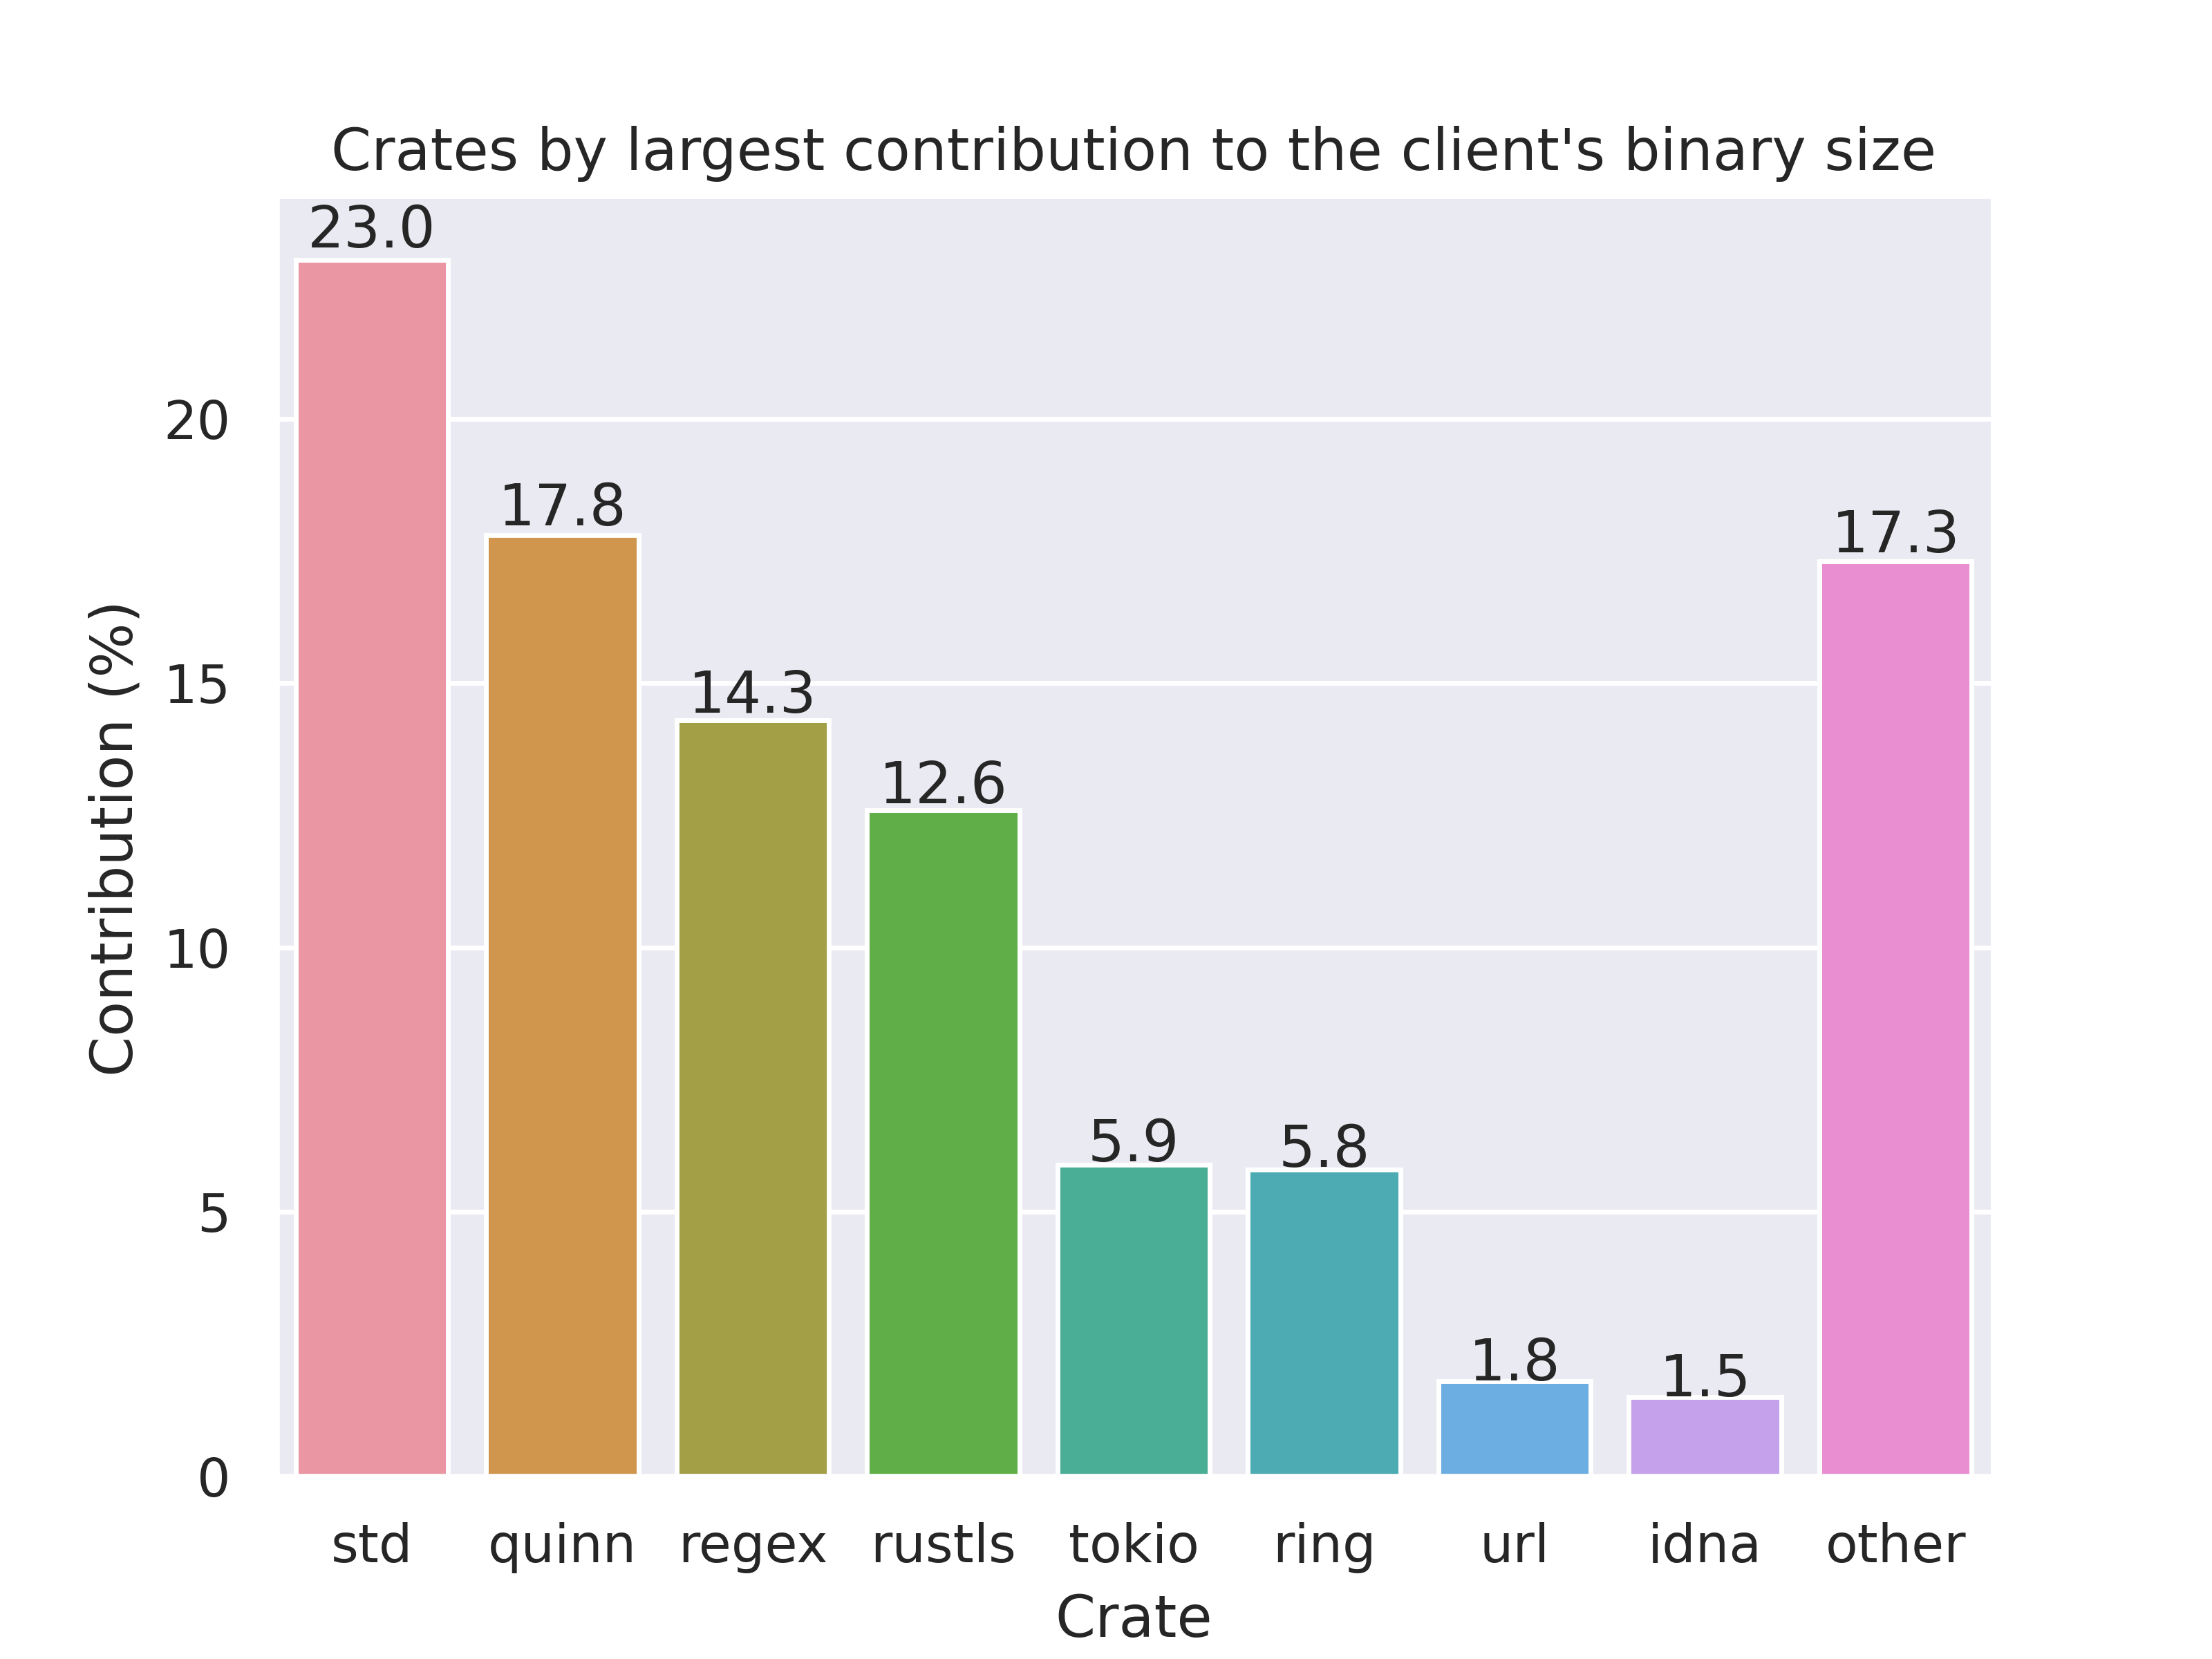
\includegraphics[width=1\linewidth]{images/mquictt_binary_client.png}
    \caption{Top contributions to the binary size of the MQuicTT client by crate. That is, which libraries contribute the largest footprint.}
    \label{fig:mquictt_client_bin}
\end{figure}

When analysing the QUIC stack contribution to the binary size we can see that $quinn$ contributes to $17.8\%$ of the binary size and $rustls$ contributes a further $12.6\%$.
Additionally, we can see that the $ring$ crate contributes another $5.8\%$.
This crate is a Rust binding for BoringSSL primitives; hence it is part of the TLS implementation.
Overall, this means that the QUIC stack constitutes $36.2\%$ of MQuicTT's client binary size.
This result is in line with our prediction that the QUIC stack will contribute the most to the size of the binary.

Unexpectedly, however, the $regex$ crate contributes $14.3\%$ to the size of the client binary exceeding even the contribution made by the TLS implementation.
This can partially be attributed to Rust's support for Unicode in strings.
Specifically, a $char$ type in Rust represents a Unicode scalar value, a Unicode version agnostic type.
While providing many wanted features, Rust's native support for Unicode also increases the used resources.
A possible workaround would be to add optional support for the $unicase::Ascii$ type to the $regex$ crate.
Another possible reason for the size of this crate is the source codes extensive use of the $inline(always)$ annotation.
This annotation tells the compiler to inline functions across crate boundaries, possibly contributing to the binary size.
Overall, we can see that this anomaly can be attributed to the choice of programming language, which presents an insight into Rust as a language for hardware constrained devices.

We can also see that despite other crates not contributing a considerable amount towards the binary size, cumulatively, their size adds up to $17.3\%$ of the binary size due to the large number of them.
We have found over 40 crates that contributed to this, including data structure implementations, lower-level network interfaces, abstractions on byte buffers and logging utilities.
Notably, we have found that logging utilities and error reporting do not largely contribute to the size of the client's binary.
This comes in contrast to one of the steps in reducing the binary size taken by~\cite{eggert_towards_2020}.

Figure~\ref{fig:mquictt_broker_bin} shows similar results for MQuicTT's broker.
We can see that in the case of the broker, the QUIC stack constitutes $32.9\%$ of the binary size.
Similarly to the client, the $regex$ crate again shows a large binary size footprint, and the lesser crates contribute to a sizeable cumulative amount.
Additionally, similarly to the results presented for the client, we have found that the logging and error checking crates have not contributed largely to the binary size.

\begin{figure}[ht]
    \centering
    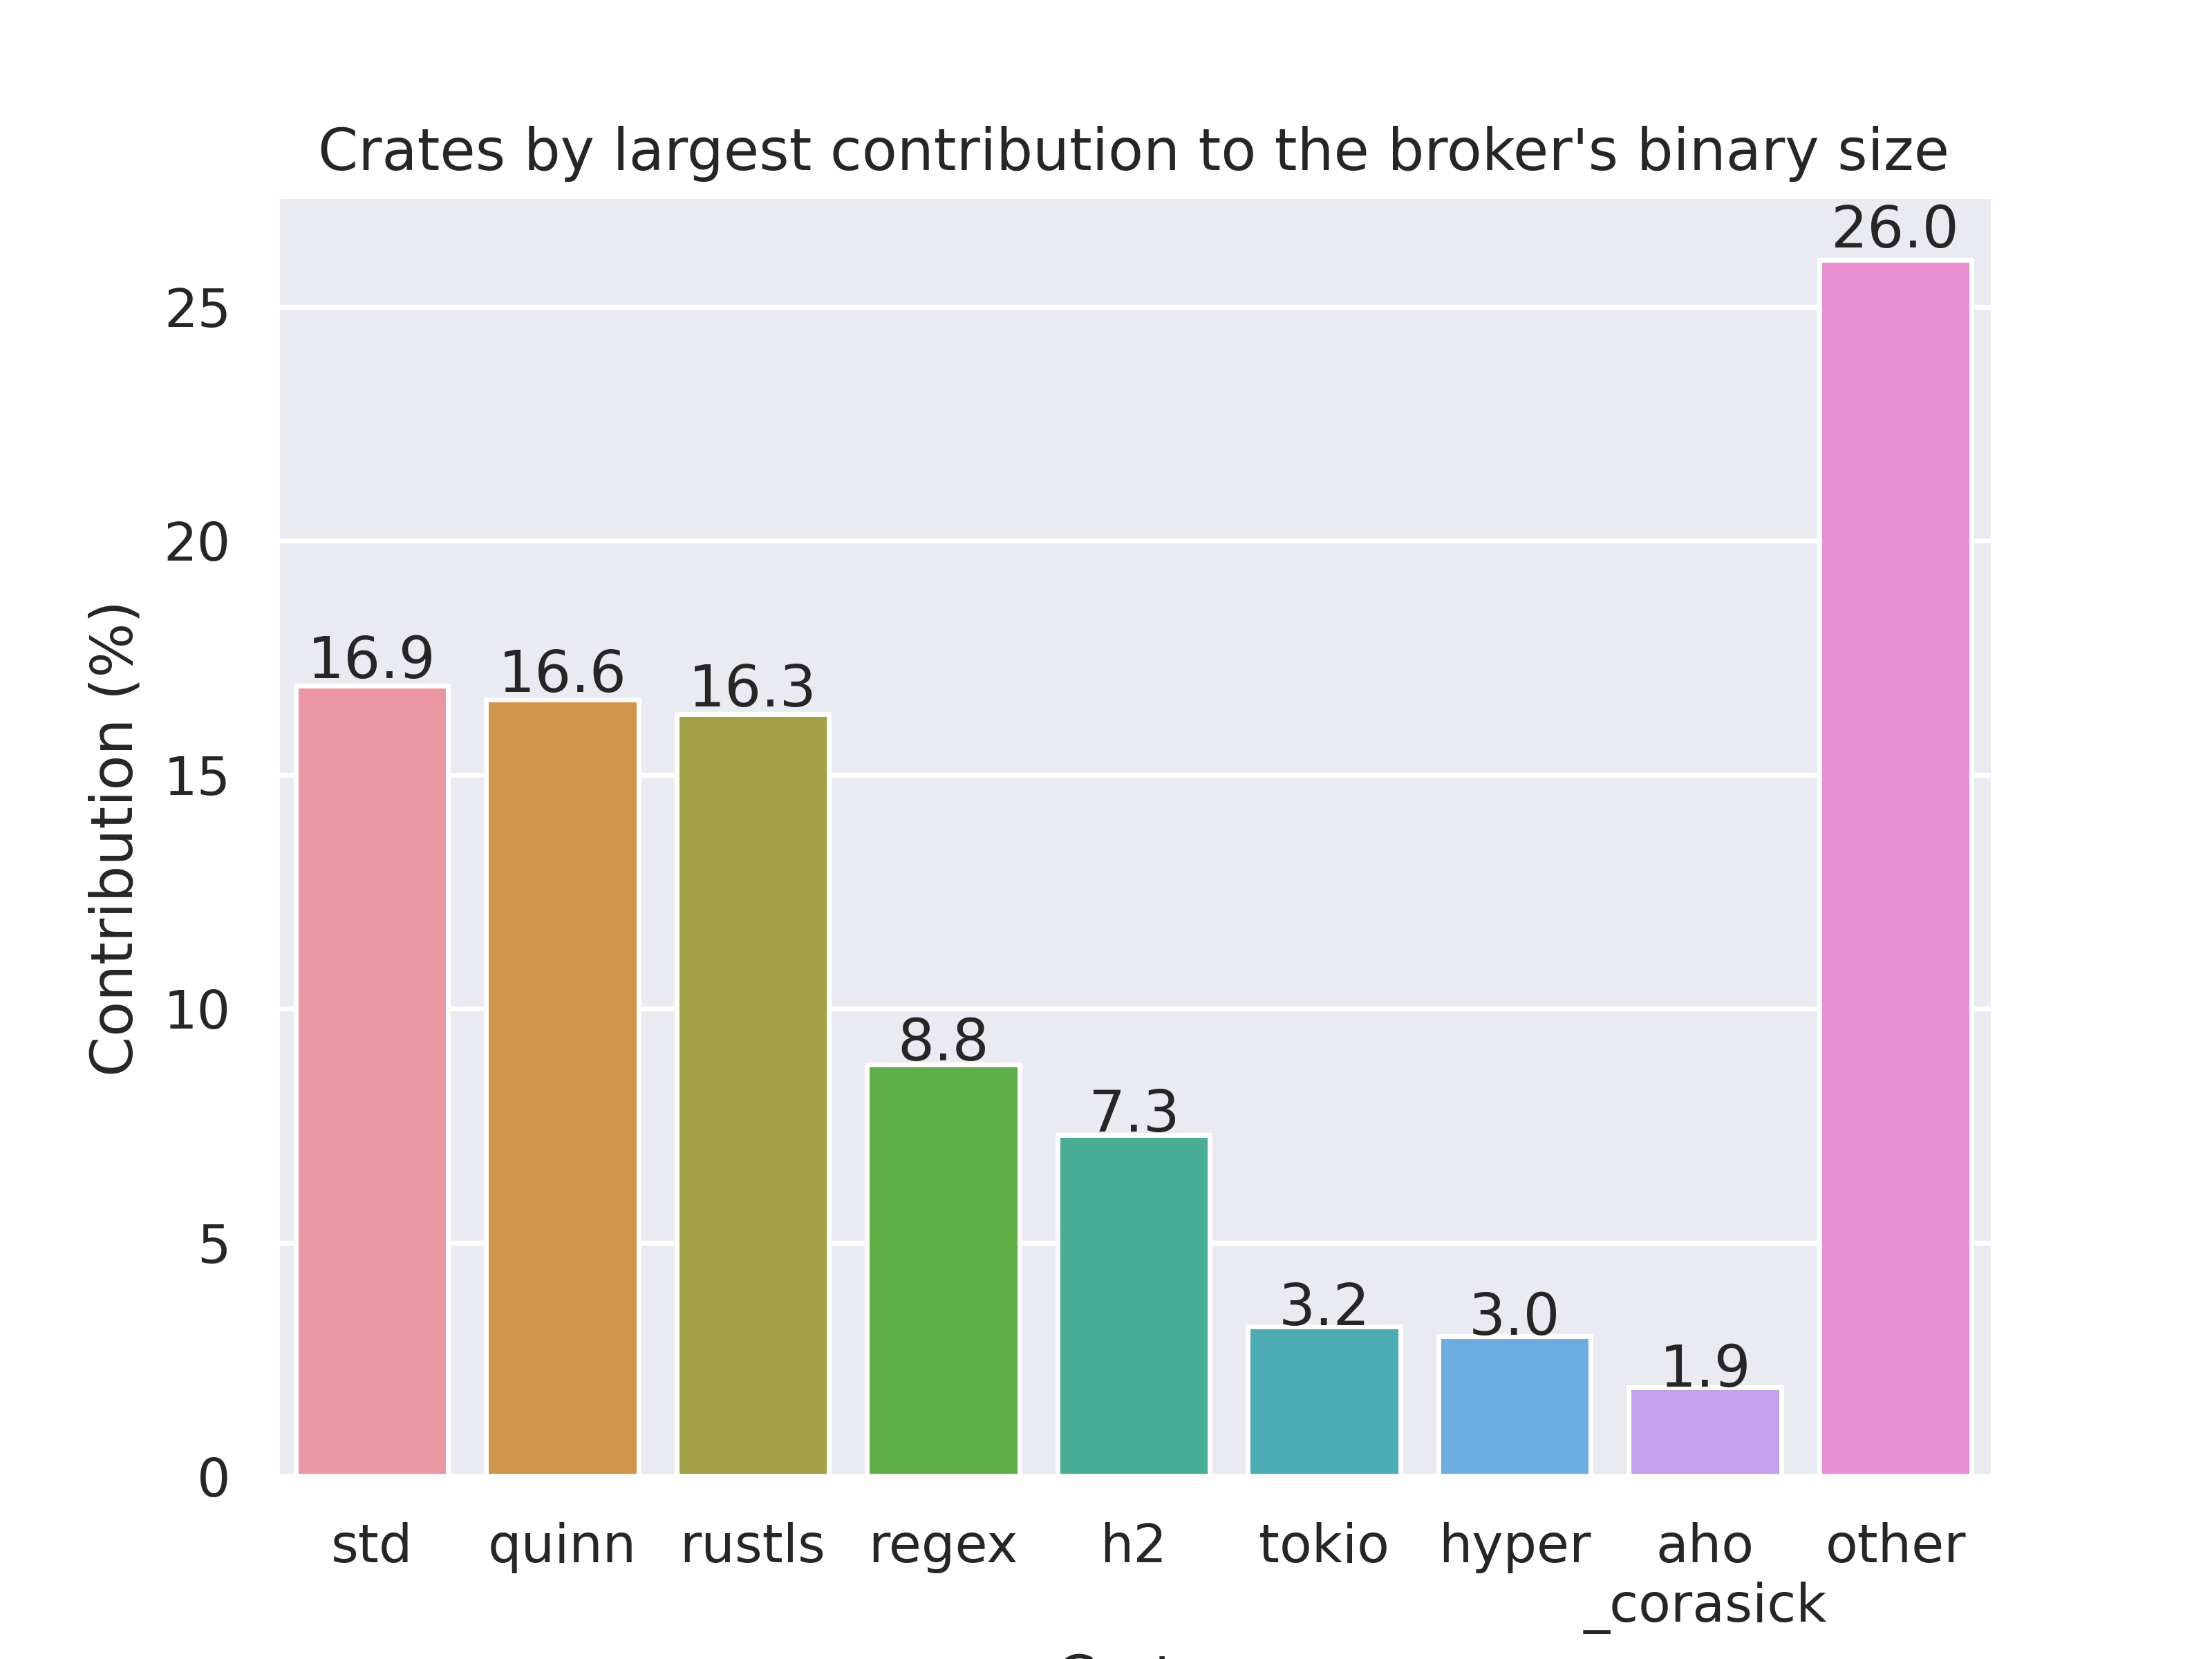
\includegraphics[width=1\linewidth]{images/mquictt_binary_broker.png}
    \caption{Top contributions to the binary size of the MQuicTT broker by crate. That is, which libraries contribute the largest footprint.}
    \label{fig:mquictt_broker_bin}
\end{figure}

We have further analysed the binary to see which methods contribute to the size for the client and broker.
Notably, in both cases, the $quinn\_proto$ module of $quinn$ contains several methods such as $connection::Connection::process\_payload$ and $endpoint::Endpoint::handle$ that each contribute around $0.8\%$.
Notably, however, the $regex::exec::ExecBuilder::build$ method from the $regex$ crate contributes $0.7\%$, which is a larger contribution than $quinn's$ methods for decrypting packets and polling for connections.

\begin{figure}
    \begin{center}
        \begin{subfigure}[b]{0.6\textwidth}
            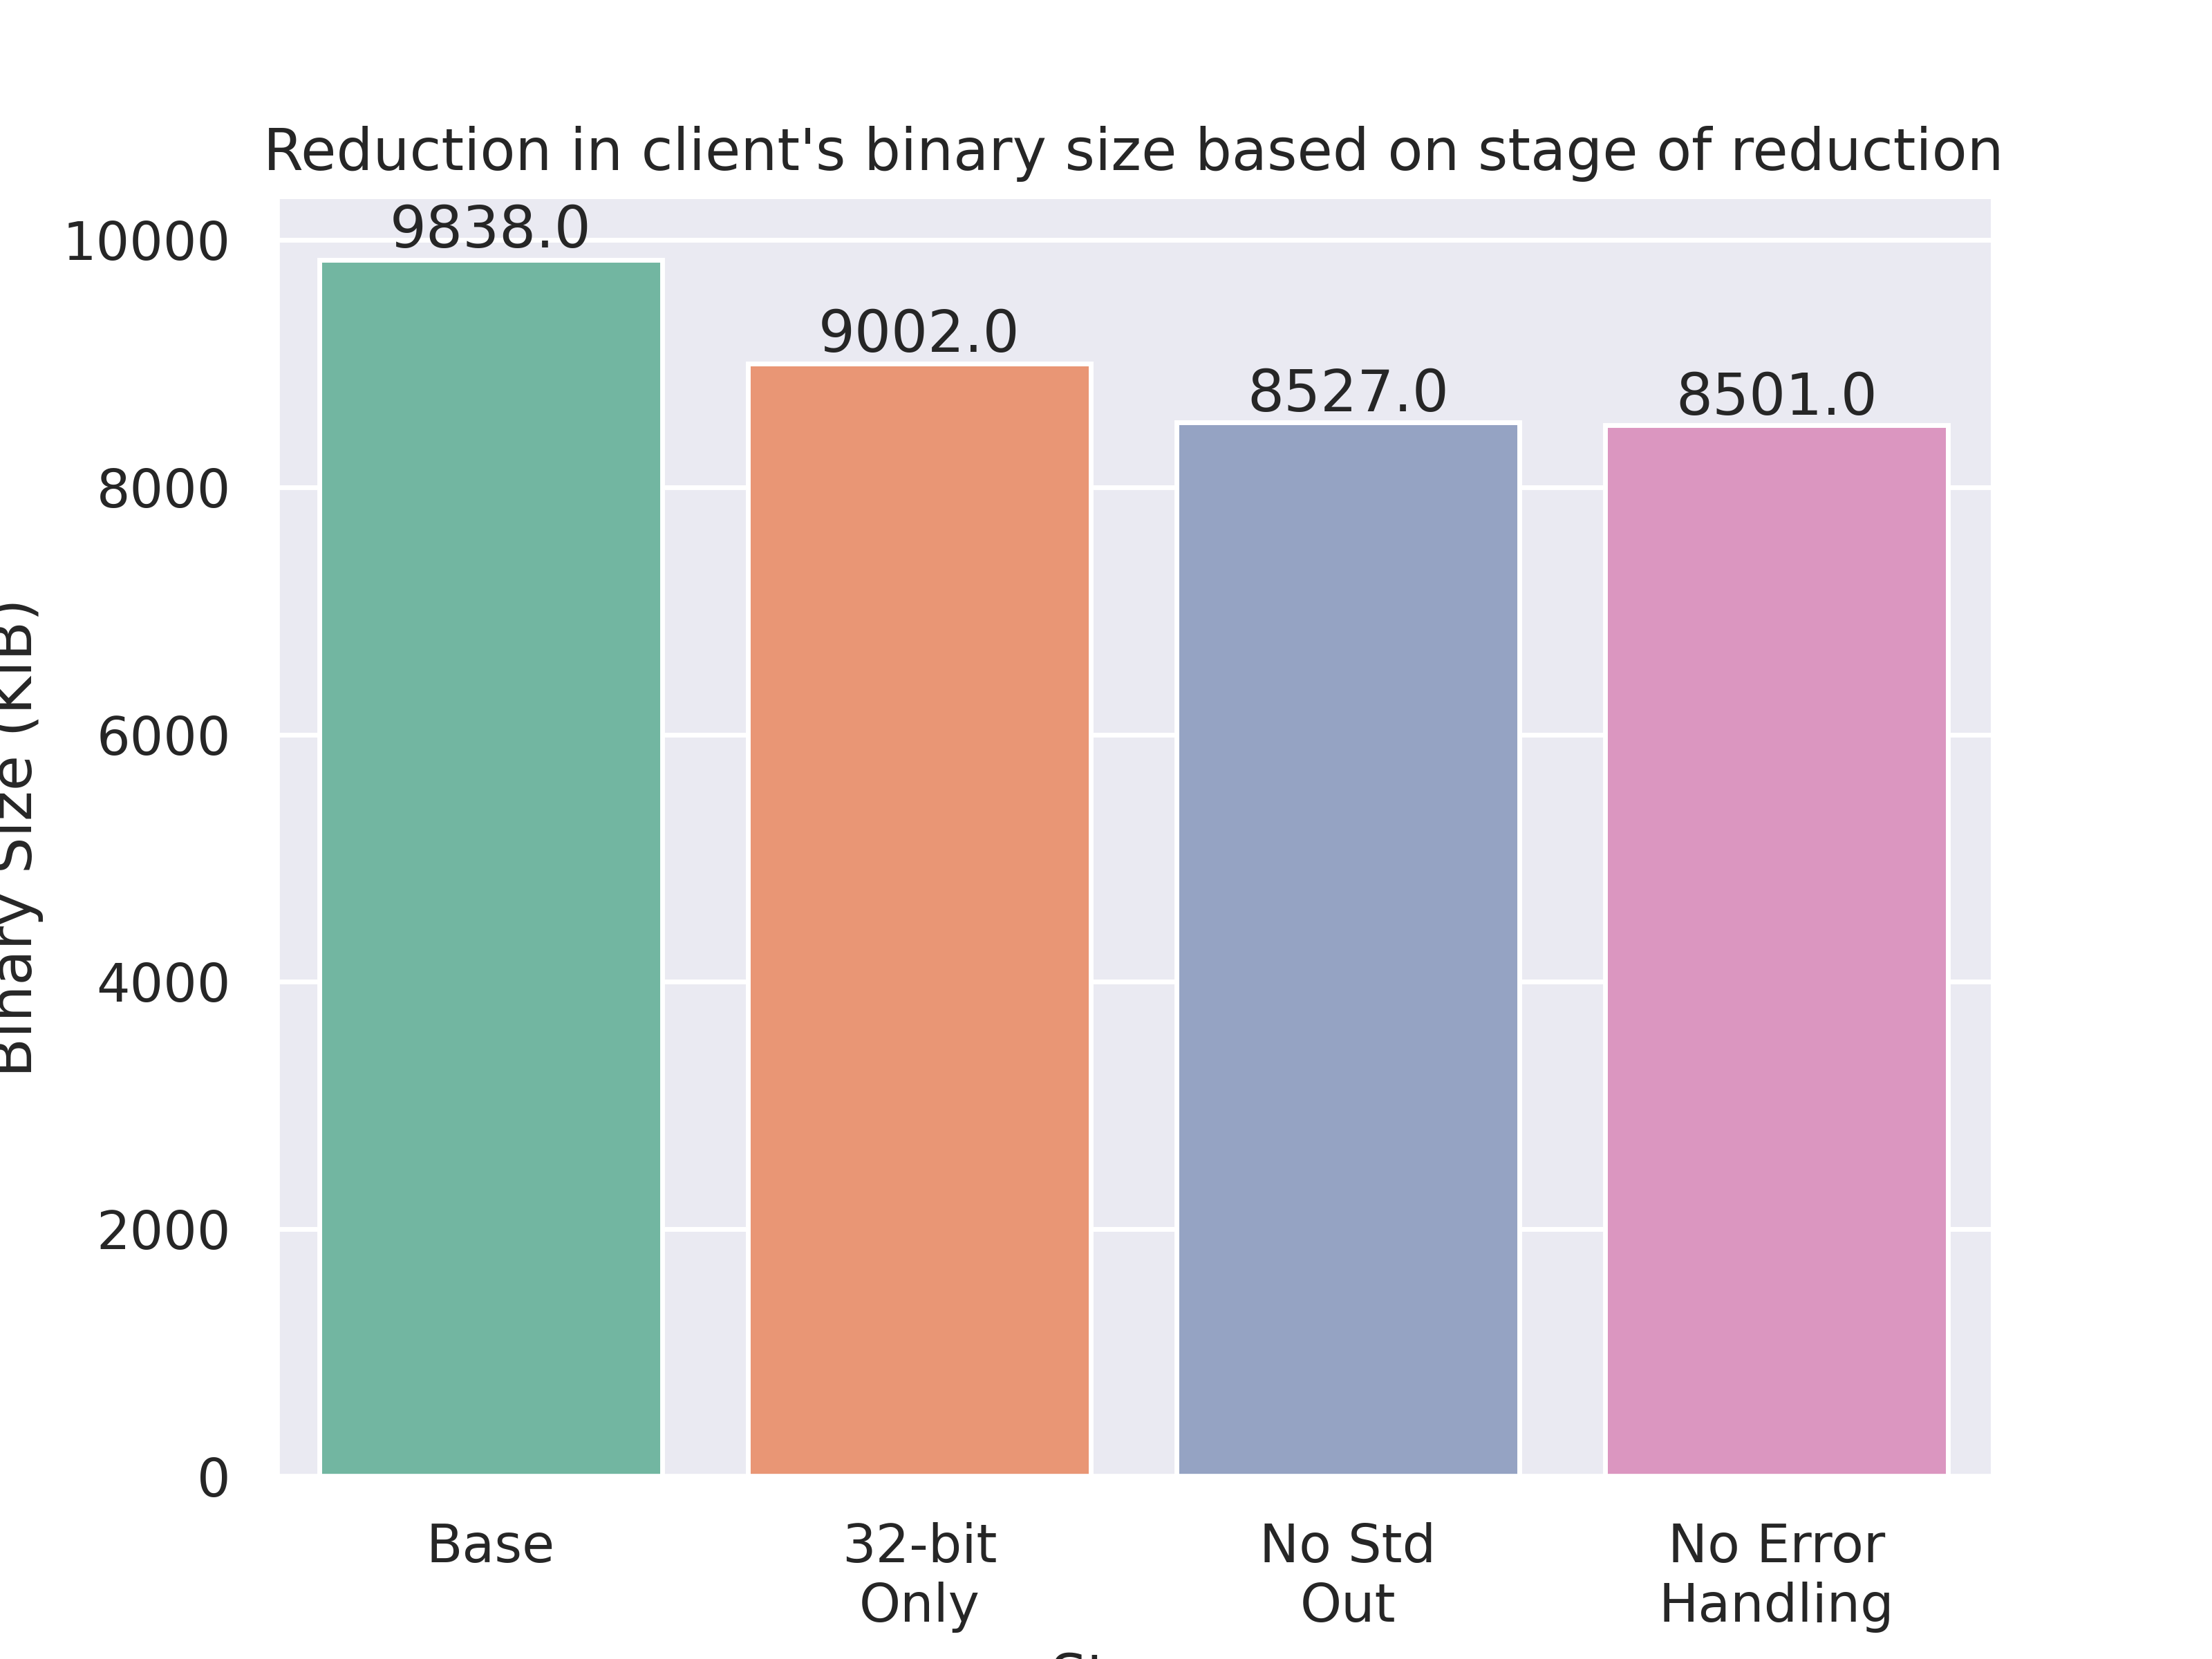
\includegraphics[width=1\linewidth]{images/quinn_binary_reduce_client.png}
            \caption{Client binary size reduction.}
            \label{fig:reduce_client}
        \end{subfigure}
        \begin{subfigure}[b]{0.6\textwidth}
            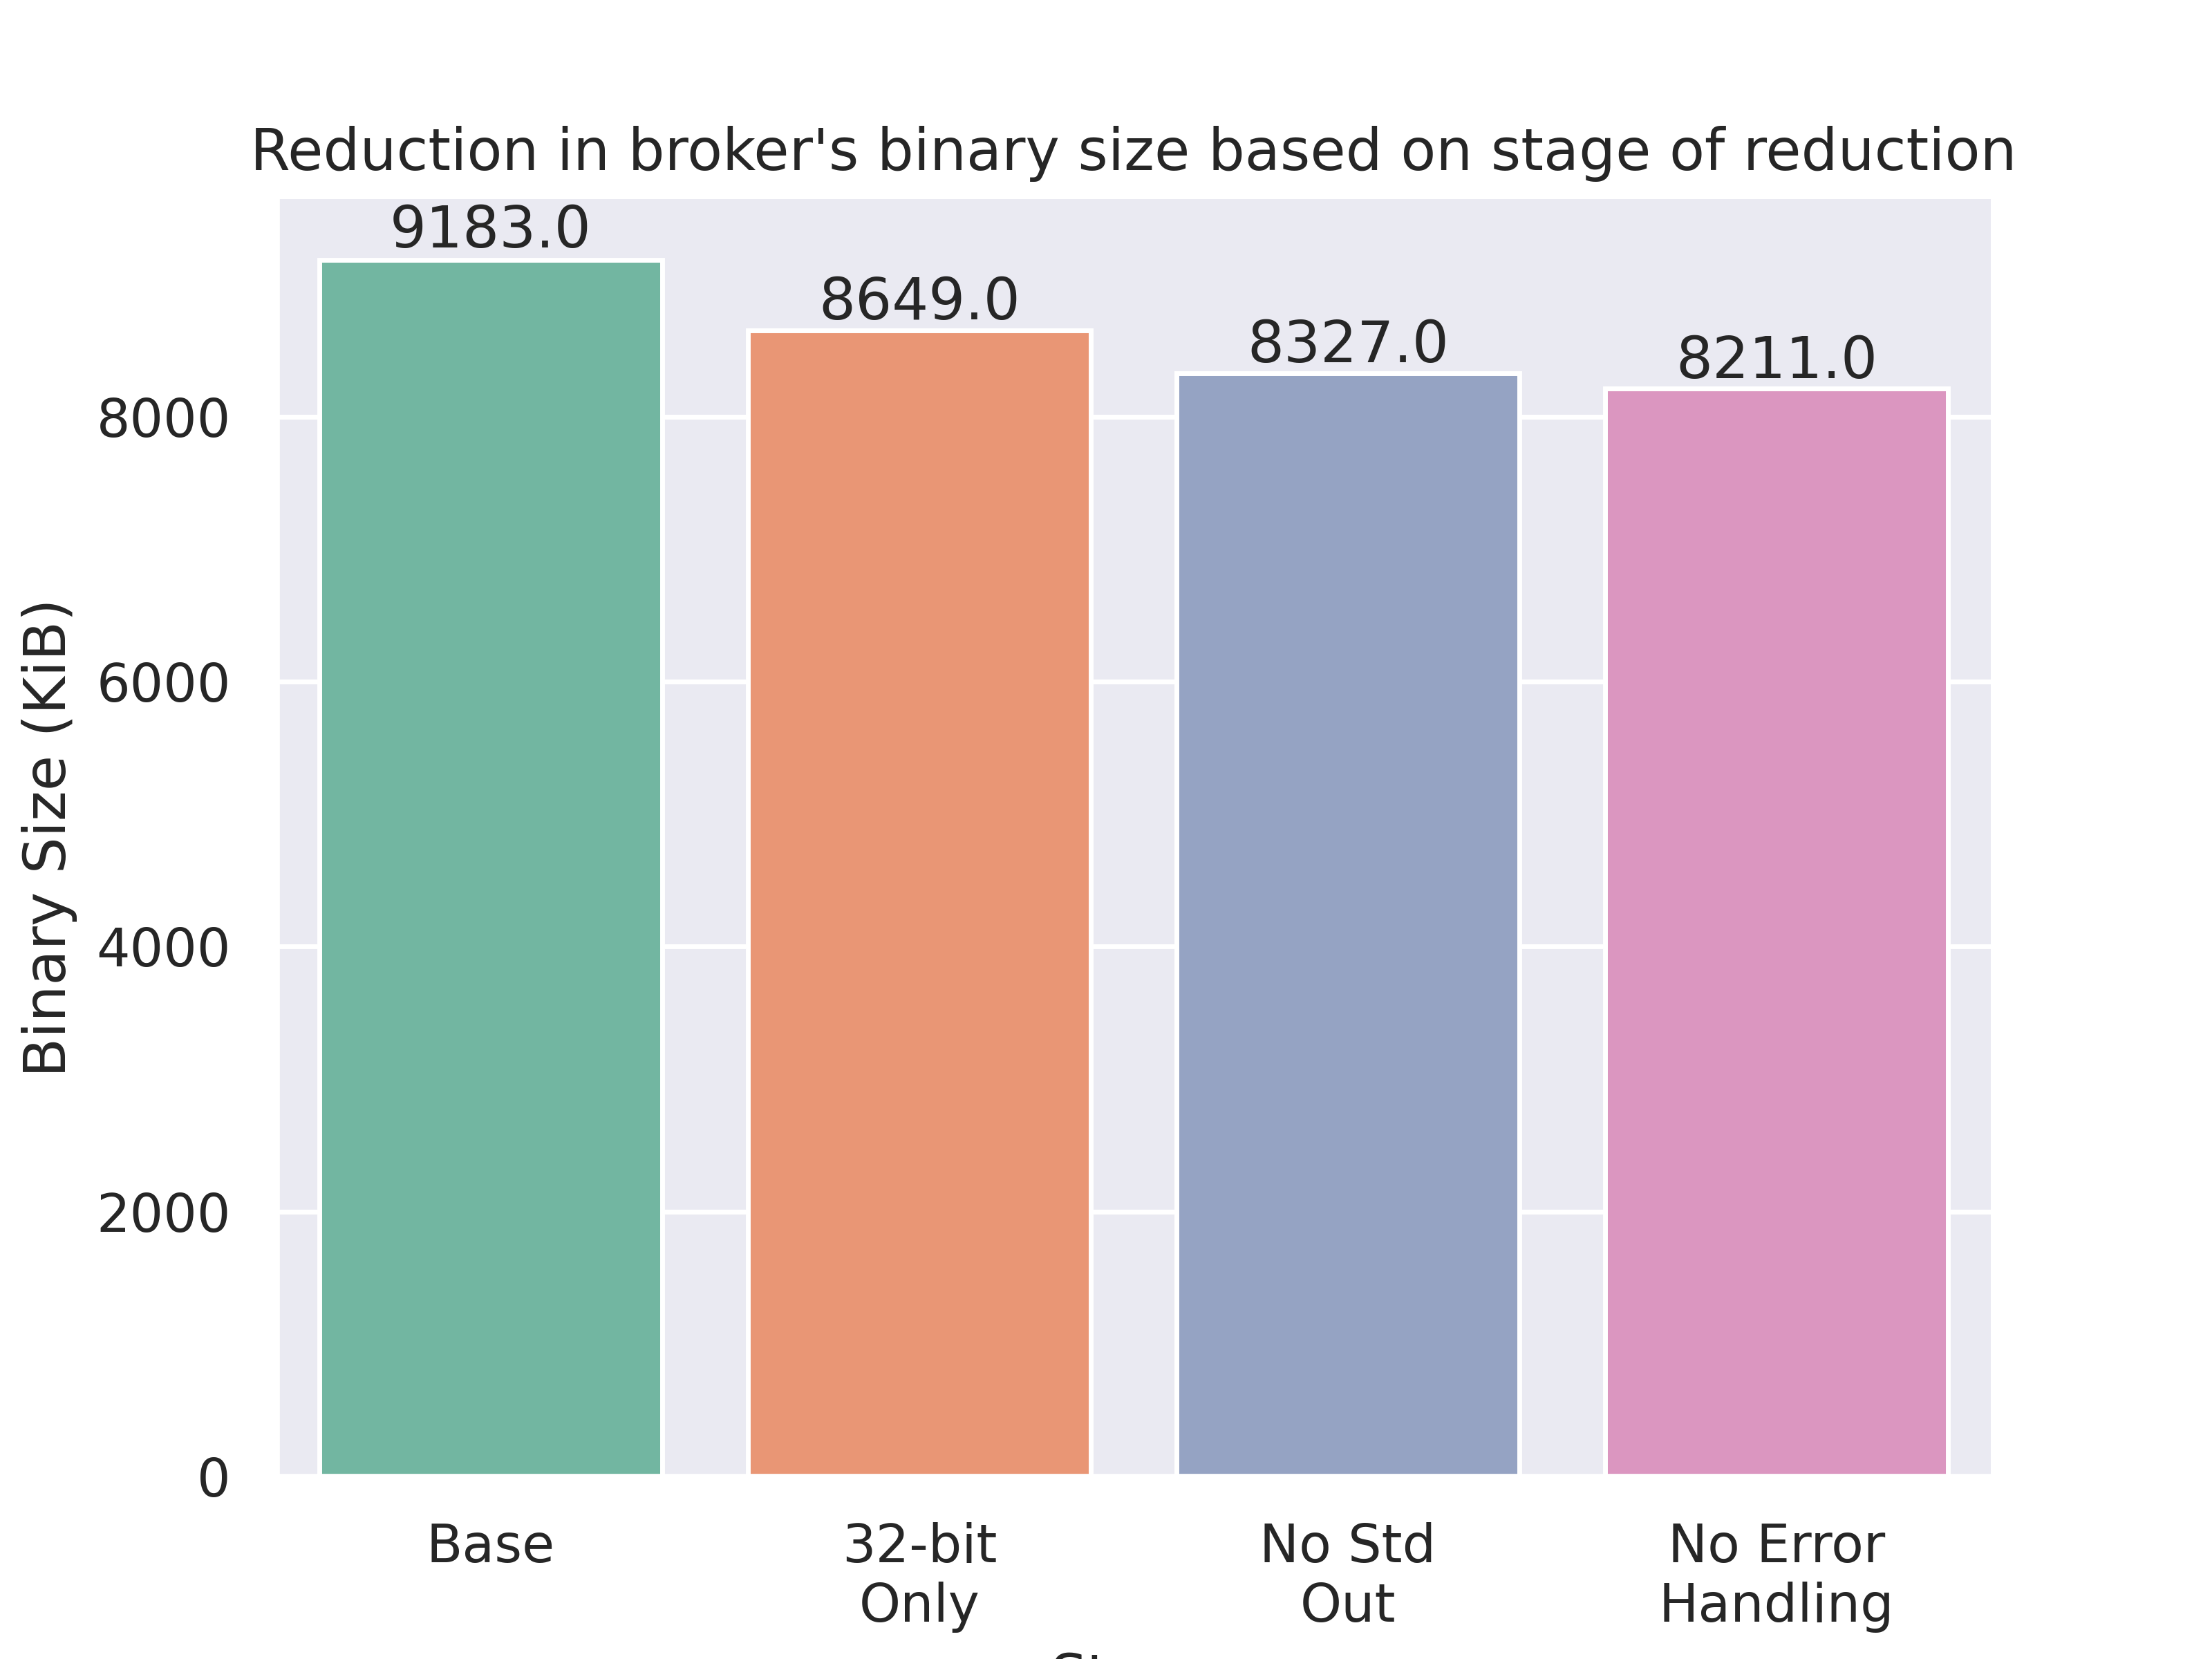
\includegraphics[width=1\linewidth]{images/quinn_binary_reduce_broker.png}
            \caption{Broker binary size reduction.}
            \label{fig:reduce_roker}
        \end{subfigure}
        \caption{The stages of the reduction and the sizes of the QUIC binary at the corresponding stages.}
        \label{fig:reduce}
    \end{center}
\end{figure}

\subsection{Reducing the QUIC stack}

As we can see from the composition of the binaries of MQuicTT, the QUIC stack is around a third of the size of the implementation.
Hence, we now analyse methods for reducing QUIC's contribution following the previously described methodology.

Figure~\ref{fig:reduce} demonstrates the reduction in binary size at each stage described in the methodology.
Notably, compiling the binary to a 32-bit only target contributes significantly to the reduction of the binary size.
The 32-bit only version of the broker is $5.8\%$ smaller and the 32-bit only client is $8.5\%$ smaller.
However, the two remaining stages did not contribute significantly to the reduction of the binary sizes.
This can perhaps be attributed to implementation details as the reduction due to error handling and standard output use would be directly proportional to their use in the code base.
This is further reinforced by the client being reduced by a higher percentage from removing error handling due to the client's source code having more of this feature.

Hence, from the binary analysis conducted we can see that the QUIC stack contributes a large amount to the overall binary size of MQuicTT.
We can also see that reducing the size of the QUIC stack is not trivial with best results coming from compiling to a 32-bit only target.

When it comes to reducing the size of the TLS component~\cite{eggert_towards_2020} attempts create a minimal cypher implementations used by TLS, and we instead opt to discuss the possibility of a complete alternative to TLS, suitable for hardware constrained devices in Section~\ref{chap:TLS}.
